\chapter{Developed work}%
\label{chap:developed-work}

% -----------------------------------------------------------------------------------------------------
\section{General Guidelines}
\label{sec:guidelines}

\begin{itemize}
    \item \textbf{File formats}: Use PDF or EPS for vector graphics (diagrams, plots), PNG or JPEG for photographs.
    \item \textbf{Cross-referencing}: Always use \texttt{\textbackslash label} and \texttt{\textbackslash ref} for all equations, tables, and figures.
    \item \textbf{Captions}: Provide both short (for list of figures/tables) and long descriptions where appropriate.
    \item \textbf{Placement}: Use \texttt{[htbp]} for flexible figure/table placement.
    \item \textbf{Units}: Use proper math mode formatting for units (e.g., m/s$^2$).
    \item \textbf{Consistency}: Maintain consistent notation throughout the document.
    \item \textbf{Spacing}: Use \texttt{\textbackslash quad} or \texttt{\textbackslash qquad} for spacing in equations.
\end{itemize}

% -----------------------------------------------------------------------------------------------------
\section{Mathematical Equations}
\label{sec:equations}

When presenting mathematical content, ensure equations are properly formatted and referenced. Use the \texttt{equation} environment for single equations and \texttt{align} for multiple lines.

\begin{equation}
    \label{eq:rotation-matrix}
    \dot{\varphi} = \frac{1}{\cos{\theta}} 
    \begin{bmatrix}
        \cos\theta & \sin\phi \sin\theta & \cos\phi \sin\theta \\
        0          & \cos\phi \cos\theta & -\sin\phi \cos\theta \\
        0          & \sin\phi             & \cos\phi
    \end{bmatrix} \omega
\end{equation}

Equation~\ref{eq:rotation-matrix} shows the relationship between angular velocities and Euler angle rates. Always introduce equations in the text before presenting them.

% -----------------------------------------------------------------------------------------------------
\section{Tables and Data Presentation}
\label{sec:tables}

Tables should be clear, self-contained, and properly formatted. Use the \href{https://www.tablesgenerator.com/}{Tables Generator} tool for assistance. Maintain consistent formatting with your thesis style.

\begin{table}[htbp]
    \centering
    \caption{Controller Design Parameters}
    \label{tbl:controller-parameters}
    \begin{tabular}{llrl}
        \toprule
        \textbf{Parameter} & &\textbf{Value} & \textbf{Unit} \\
        \midrule
        Maximum acceleration &$a_{\mathrm{max}}$ & 1.0 & m/s$^2$ \\
        Maximum angular rate &$q_{\mathrm{max}}$ & 1.0 & rad/s \\
        Maximum bank angle &$\eta_{\mathrm{max}}$ & 6.0 & $^\circ$ \\
        \bottomrule
    \end{tabular}
\end{table}

Table~\ref{tbl:controller-parameters} summarizes the key design parameters. Always reference tables in the text and use consistent terminology.

% -----------------------------------------------------------------------------------------------------
\section{Figures and Visual Elements}
\label{sec:figures}

Figures enhance understanding of complex concepts. Include clear captions and proper references. For TikZ diagrams, consider using direct input for better integration. Figure~\ref{fig:control-block} illustrates the structure of a typical feedback control system. For vector graphics, PDF format is preferred.


\begin{figure}[H]
    \centering
    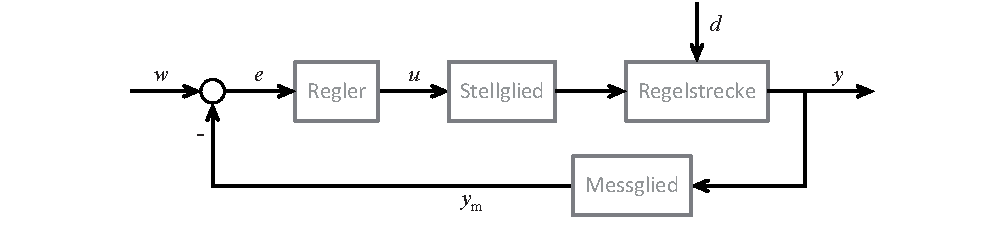
\includegraphics[width=\textwidth]{./src/pics/Regelkreis.pdf}
    \caption[Block diagram of a control system]{Block diagram of a feedback control system showing the basic components: plant, controller, and feedback loop.}
    \label{fig:control-block}
\end{figure}


For complex diagrams created with TikZ/PGF, you can include them directly:

\begin{figure}[H]
    \centering
    % !TeX root = ../../Main.tex
\tikzstyle{block} = [draw, fill=cyan!100, rectangle, 
    minimum height=10mm, minimum width=20mm]
\tikzstyle{sum} = [draw, fill=cyan!100, circle, inner sep=1.0mm , node distance=1cm]
\begin{tikzpicture}[auto, node distance=30mm,>={Latex[length=6pt]}]     
    \node [name=input] {};
    \node [sum, right of=input] (sum) {};
    \node [block, right of=sum,node distance=35mm] (system) {\Large$\boldsymbol{G}$};
    \node [below of=system,node distance=8mm] (slabel) {plant};
    \node [below left of=system,node distance=30mm] (controller_ref) {} ;
    \node [block, right of=controller_ref,node distance=3mm] (controller) {\Large$\boldsymbol{K}$} ;
    \node [below of=controller,node distance=8mm] (clabel) {controller};
    \node [right of=system,node distance=40mm] (output) {};      
    \node [block, right of=controller,node distance=32mm] (filter) {\Large$\boldsymbol{F}$};
    \node [below of=filter,node distance=8mm] (flabel) {filter};

    \draw [draw,->] (input) -- node {$\boldsymbol w$} (sum);
    \draw [->] (sum) -- node[pos=0.5] {$\boldsymbol u$} (system);
    \draw [->] (system) -- node [name=y,pos=0.75] {$\boldsymbol y$}(output);
    \draw [->] (y) |- (filter);
    \draw [->] (filter) -- node[pos=0.4] {$\boldsymbol y_{filt}$} (controller);
    \draw [->] (controller) -| node[pos=0.92] {$-$} node [near end] {$\boldsymbol w_{ctr}$} (sum);
\end{tikzpicture}
    \caption{Controller with pre-filter structure}
    \label{fig:controller-filter}
\end{figure}

\subsection{Multiple Images with Shared Caption}
\label{subsec:subfigures}

When you need to show related images that should share a single caption with individual sub-captions, use the \texttt{subfigure} environment. This is ideal for comparing different views, stages, or aspects of your work.

\begin{figure}[H]
    \centering
    \begin{subfigure}{.4\textwidth}
        \centering
        \includegraphics[width=\textwidth]{example-image-a}
        \caption{Front view of the satellite.}
        \label{fig:sat-front}
    \end{subfigure}
    \hfill
    \begin{subfigure}{.4\textwidth}
        \centering
        \includegraphics[width=\textwidth]{example-image-b}
        \caption{Rear view showing connectors.}
        \label{fig:sat-rear}
    \end{subfigure}
    \caption[Short description]{Long description}
    \label{fig:subfigure_env}
\end{figure}

